% Intended LaTeX compiler: xelatex
\documentclass[a4paper, 12pt]{article}
\usepackage{graphicx}
\usepackage{longtable}
\usepackage{wrapfig}
\usepackage{rotating}
\usepackage[normalem]{ulem}
\usepackage{amsmath}
\usepackage{amssymb}
\usepackage{capt-of}
\usepackage{hyperref}
\usepackage[danish]{babel}
\usepackage{mathtools}
\usepackage[margin=3.0cm]{geometry}
\hypersetup{colorlinks, linkcolor=black, urlcolor=blue}
\setlength{\parindent}{0em}
\parskip 1.5ex
\author{Jacob Debel}
\date{Fysik C \& B}
\title{Lys og bølger\\\medskip
\large Rekonstruktion - Det optiske gitter}
\hypersetup{
 pdfauthor={Jacob Debel},
 pdftitle={Lys og bølger},
 pdfkeywords={},
 pdfsubject={},
 pdfcreator={Emacs 29.4 (Org mode 9.6.15)}, 
 pdflang={Danish}}
\begin{document}

\maketitle


\section*{Plane bølger}
\label{sec:org8f33e94}
\begin{minipage}{0.3\linewidth}
\begin{itemize}
\item Hvad er plane bølger?
\end{itemize}
\end{minipage}
\vline
\begin{minipage}{0.68\linewidth}
\begin{center}
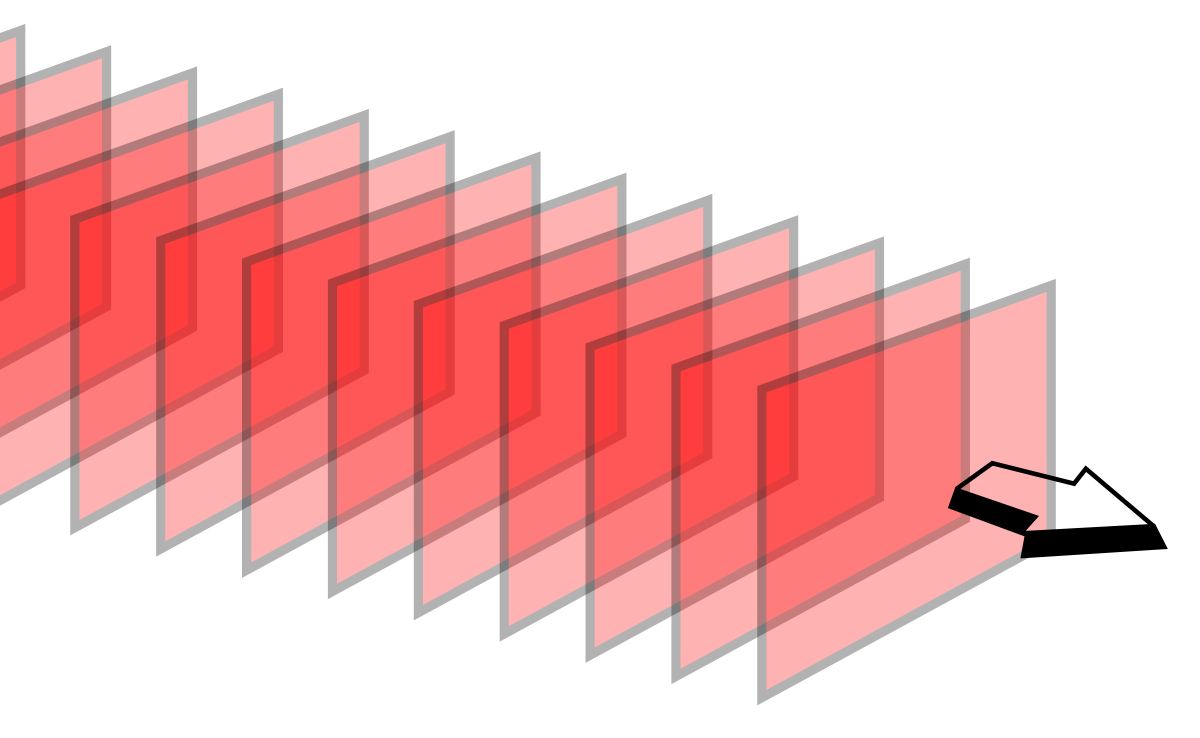
\includegraphics[width=.9\linewidth]{./img/plan_boelge.png}
\end{center}
\end{minipage}



\vfill

\begin{minipage}{0.3\linewidth}
\begin{itemize}
\item Hvornår kan ringbølger(kuglebølger) betragtes som plane bølger?
\end{itemize}
\end{minipage}
\vline
\begin{minipage}{0.68\linewidth}
\begin{center}
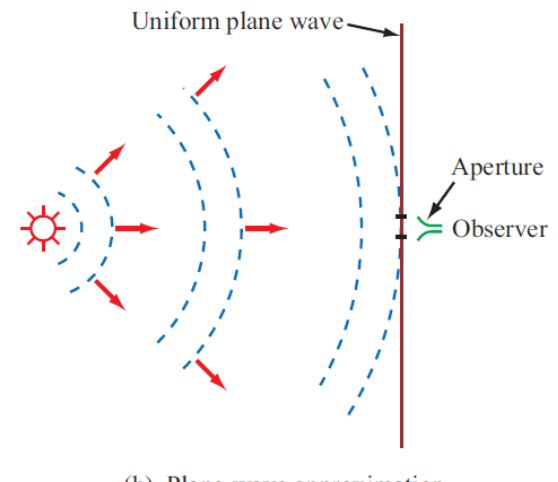
\includegraphics[width=.9\linewidth]{./img/ring_og_plane_boelger.png}
\end{center}
\end{minipage}

\vfill

\newpage
\section*{Huygens princip}
\label{sec:orgd360dc2}

\begin{minipage}{0.3\linewidth}
\begin{itemize}
\item Hvordan lyder Huygens' princip?
\end{itemize}
\end{minipage}
\vline
\begin{minipage}{0.68\linewidth}
\begin{center}
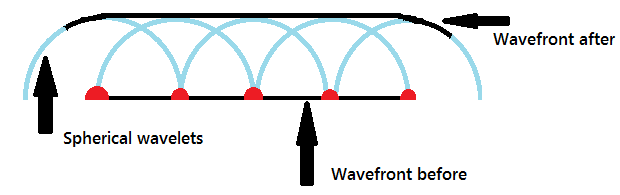
\includegraphics[width=.9\linewidth]{./img/huygens.png}
\end{center}
\end{minipage}

\vfill

\section*{Det optiske gitter}
\label{sec:orgb8189c3}
\begin{minipage}{0.3\linewidth}
\begin{itemize}
\item Hvad er \(d\), \(n\) og \(\phi_n\) og deres enheder?
\end{itemize}
\end{minipage}
\vline
\begin{minipage}{0.68\linewidth}

\end{minipage}


\vfill

\begin{minipage}{0.3\linewidth}
\begin{itemize}
\item Hvordan indtegnes bølgefronterne til 0., 1. og 2. ordens afbøjningerne?

\item Hvor skal \(d\), \(\phi_0\), \(\phi_1\) og \(\phi_2\) være på figuren?
\end{itemize}
\end{minipage}
\vline
\begin{minipage}{0.68\linewidth}
\begin{center}
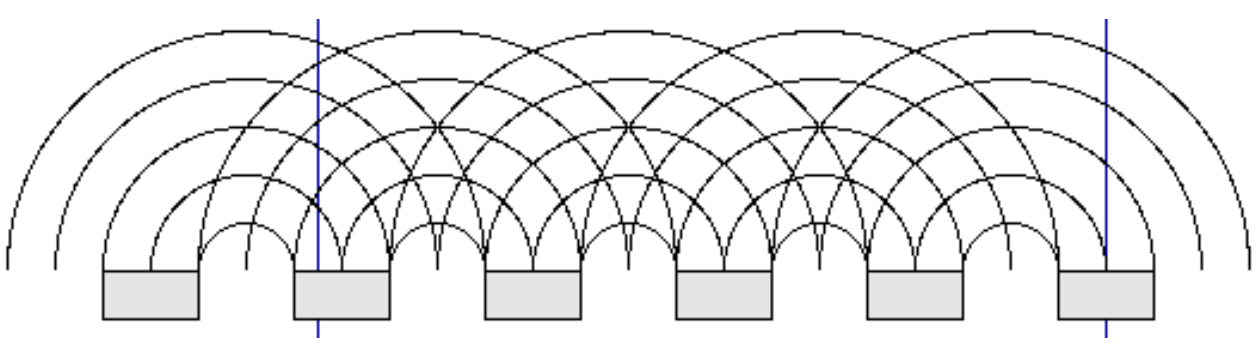
\includegraphics[width=.9\linewidth]{./img/gitter.png}
\end{center}
\end{minipage}

\vfill
\end{document}
